We are now ready to describe our construction of hub labels for CSP queries, or more specifically, for computing efficient paths. 
%We want to develop a data-structure that supports fast queries for \emph{efficient paths}. 

In Section \ref{ssec:hldef} we discussed that in case of hub labels for SP queries, if a graph $G$ has HD $h$, we can simultaneously bound the preprocessing time, storage requirements and query time as functions of $h$.
This suggests that for the CSP problem, we need an analogous property for the set of \emph{efficient paths}.
\begin{definition}[Constrained Highway Dimension] The constrained highway dimension (CHD) of $(G,\ell,c)$, denoted $h_c$, is the HD of the efficient-path system $\PE$.
\end{definition}
\noindent Note that since every shortest path is efficient, and thus $h_c\geq h$.
%, where $h$ is the HD of $G$ under shortest paths.

We now have two main issues with this definition: $(i)$ it is unclear how this can be used to get hub labels, and $(ii)$ it is unclear how the corresponding hub labels compare with those for shortest-path computations. 
To address the first question, in \cref{ssec:aug}, we reduce CSP queries in $G$ to shortest path computations in a larger \emph{augmented graph}, and use this to construct hub labels for CSP queries whose storage and query complexity can be bounded as $Bh_c$ (which can be strengthened further to $g(b)h_c$, where $g(b)$ measures the size of the Pareto frontier, cf. \cref{sec:frontier}). 
Next, in \cref{ssec:hdvschd}, we show that the hub labels for CSP queries can in fact be related to the hub labels for SP queries under an additional natural condition on the efficient paths.
Finally, in \cref{sec:avg_hd}, we study average-case guarantees on hub-label sizes, and show how in this regime, we can obtain stronger and more interpretable bounds linking the average HD and CHD.

\subsection{Hub Labels For CSP}
\label{ssec:aug}

To link the CHD to hub labels, we first convert the original graph $(G,\ell,c)$ into an \emph{augmented graph} $G^B$ with only edge lengths, such that the \emph{efficient paths of $G$ are in bijection with the shortest paths of $G^B$}. We note that our reduction follows standard dynamic programming arguments; similar approaches have been proposed for CSP~\cite{alex_bicriteria}, albeit without preprocessing.


Our construction is as follows: each node in $G^B$ is of the form $\pp{v,b}$, jointly encoding the location $v\in V$ and remaining budget $b\geq 0$.
A node is connected to neighbors (according to $E$) as long as the remaining budget of that transition is non-negative.
Finally, we create $n$ sink nodes, denoted $v^-$, and connect node $\pp{v,b}$ to $v^-$ with length $1/(b+1)$.
An illustration of the construction is presented in \cref{fig:augmented}.
Paths in $G^B$ are mapped back to paths in $G$ by removing the budget labels and sink nodes.
We call this mapping the \emph{projection} of a path.
%Finally, assuming we use that in $G^B$ paths consuming more budget are penalized, we can prove the following.
Now we have the following:

%\begin{definition}[Augmented Graph]
%Given $(G,\ell,c)$ and $B\in\N$, the augmented version $G^B$ has vertex set\\
%$V^B \defeq\crl*{\pp{v,b}: v\in V, b=0,1,\ldots,B}\cup\crl*{v^-:v\in V}$, the edge set $E^B$ contains $\crl*{\pp{v,b}\pp{w,x} : vw\in E, x=b-c_{vw}, x\geq 0}$ with the additional $\crl*{\pp{v,b}v^-: v\in V, 0\leq b\leq B}$.
%The length function in $G^B$ is $\ell(\pp{v,b},v^-) \defeq \frac{1}{b+1}$ and $\ell(\pp{v,b},\pp{w,x}) \defeq \ell(vv')$.
%\end{definition}

\begin{figure}
	\begin{center}
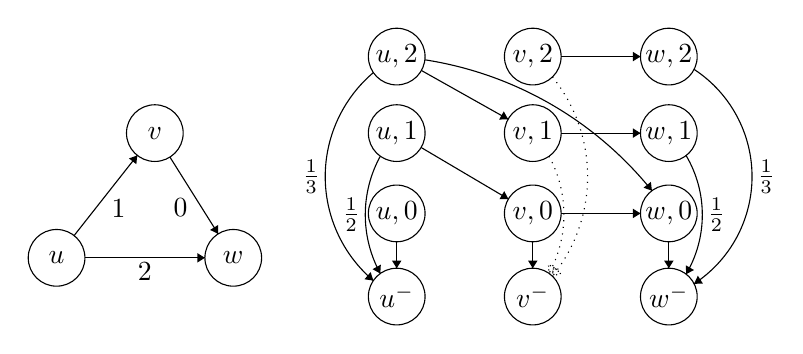
\begin{tikzpicture}[scale=0.12]
\tikzstyle{every node}+=[inner sep=0pt]
\draw [black] (5,-34.3) circle (3);
\draw (5,-34.3) node {$u$};
\draw [black] (15.4,-21.1) circle (3);
\draw (15.4,-21.1) node {$v$};
\draw [black] (23.7,-34.3) circle (3);
\draw (23.7,-34.3) node {$w$};
\draw [black] (41,-13) circle (3);
\draw (41,-13) node {$u,2$};
\draw [black] (41,-21.1) circle (3);
\draw (41,-21.1) node {$u,1$};
\draw [black] (41,-29.6) circle (3);
\draw (41,-29.6) node {$u,0$};
\draw [black] (41,-38.4) circle (3);
\draw (41,-38.4) node {$u^-$};
\draw [black] (55.4,-13) circle (3);
\draw (55.4,-13) node {$v,2$};
\draw [black] (55.4,-21.1) circle (3);
\draw (55.4,-21.1) node {$v,1$};
\draw [black] (55.4,-29.6) circle (3);
\draw (55.4,-29.6) node {$v,0$};
\draw [black] (55.4,-38.4) circle (3);
\draw (55.4,-38.4) node {$v^-$};
\draw [black] (69.8,-13) circle (3);
\draw (69.8,-13) node {$w,2$};
\draw [black] (69.8,-21.1) circle (3);
\draw (69.8,-21.1) node {$w,1$};
\draw [black] (69.8,-29.6) circle (3);
\draw (69.8,-29.6) node {$w,0$};
\draw [black] (69.8,-38.4) circle (3);
\draw (69.8,-38.4) node {$w^-$};
\draw [black] (6.86,-31.94) -- (13.54,-23.46);
\fill [black] (13.54,-23.46) -- (12.66,-23.78) -- (13.44,-24.39);
\draw (10.77,-29.12) node [right] {$1$};
\draw [black] (17,-23.64) -- (22.1,-31.76);
\fill [black] (22.1,-31.76) -- (22.1,-30.82) -- (21.25,-31.35);
\draw (18.92,-29) node [left] {$0$};
\draw [black] (8,-34.3) -- (20.7,-34.3);
\fill [black] (20.7,-34.3) -- (19.9,-33.8) -- (19.9,-34.8);
\draw (14.35,-34.8) node [below] {$2$};
\draw [black] (43.98,-13.342) arc (81.20715:38.87551:38.409);
\fill [black] (68.01,-27.19) -- (67.9,-26.26) -- (67.12,-26.88);
\draw [black] (43.58,-22.62) -- (52.82,-28.08);
\fill [black] (52.82,-28.08) -- (52.38,-27.24) -- (51.87,-28.1);
\draw [black] (58.4,-29.6) -- (66.8,-29.6);
\fill [black] (66.8,-29.6) -- (66,-29.1) -- (66,-30.1);
\draw [black] (43.61,-14.47) -- (52.79,-19.63);
\fill [black] (52.79,-19.63) -- (52.33,-18.8) -- (51.84,-19.67);
\draw [black] (58.4,-21.1) -- (66.8,-21.1);
\fill [black] (66.8,-21.1) -- (66,-20.6) -- (66,-21.6);
\draw [black] (58.4,-13) -- (66.8,-13);
\fill [black] (66.8,-13) -- (66,-12.5) -- (66,-13.5);
\draw [black] (72.471,-14.353) arc (56.79859:-56.79859:13.561);
\fill [black] (72.47,-37.05) -- (73.41,-37.03) -- (72.87,-36.19);
\draw (79.11,-25.7) node [right] {$\frac{1}{3}$};
\draw [black] (71.625,-23.471) arc (30.61438:-30.61438:12.329);
\fill [black] (71.63,-36.03) -- (72.46,-35.59) -- (71.6,-35.09);
\draw (73.84,-29.75) node [right] {$\frac{1}{2}$};
\draw [black] (69.8,-32.6) -- (69.8,-35.4);
\fill [black] (69.8,-35.4) -- (70.3,-34.6) -- (69.3,-34.6);
\draw [black] (38.528,-36.71) arc (-130.31667:-229.68333:14.439);
\fill [black] (38.53,-36.71) -- (38.24,-35.81) -- (37.59,-36.57);
\draw (32.93,-25.7) node [left] {$\frac{1}{3}$};
\draw [black] (39.265,-35.961) arc (-151.22419:-208.77581:12.903);
\fill [black] (39.26,-35.96) -- (39.32,-35.02) -- (38.44,-35.5);
\draw (37.17,-29.75) node [left] {$\frac{1}{2}$};
\draw [black] (41,-32.6) -- (41,-35.4);
\fill [black] (41,-35.4) -- (41.5,-34.6) -- (40.5,-34.6);
\draw [black] (55.4,-32.6) -- (55.4,-35.4);
\fill [black] (55.4,-35.4) -- (55.9,-34.6) -- (54.9,-34.6);
\draw [dotted] (57.481,-15.155) arc (38.87983:-38.87983:16.799);
\draw [densely dotted] (57.48,-36.24) -- (58.37,-35.94) -- (57.59,-35.31) -- cycle;
\draw [dotted] (57.121,-23.549) arc (28.47781:-28.47781:13.004);
\draw [densely dotted] (57.12,-35.95) -- (57.94,-35.49) -- (57.06,-35.01) -- cycle;
\end{tikzpicture}
\end{center}
	\caption{Example of a graph augmentation: The original graph $G$ has all paths of unit length, and costs as labeled on the edges. In the augmented graph $G^B$, the labels represent the edge lengths (unlabeled edges have length 1). Note the additional edges from $(w,b)$ to the sink node $w^-$ (and similarly for $u$ and $v$). 
	}
	\label{fig:augmented}
\end{figure}


%\begin{definition}
%Let $P$ be a path in $G^B$.
%If $P$ is of the form $\pp{v_1,b_1}\ldots\pp{v_k,b_k}$, then the projection of $P$, denoted $\bar P$, is the path $\bar P\defeq v_1v_2\ldots v_k$.
%Analogously, if $P$ is of the form $\pp{v_1,b_1}\ldots\pp{v_k,b_k}v_{k}^-$, then $\bar P\defeq v_1\ldots v_{k}$. 
%\end{definition}


\begin{proposition}\label{prop:shorteffic}
	A shortest path from source $\pp{s,b}$ to sink node~$t^-$ projects to an efficient path in $G$ solving $\dist(s,t|b)$. 
\end{proposition}
%\begin{proof}
%Let $P$ be the shortest path from $\pp{s,b}$ to $t^-$, and $\bar P$ its projection.
%To reach $t^-$, $P$ must pass through some $\pp{t,b'}$, $b'\geq 0$.
%By construction, $P$ consumes $b-b'$ units of resource, hence it is feasible; moreover, $\bar P$ is the shortest among $(s,t)$-paths with cost $b-b'$.
%Now assume, by way of contradiction, that $\bar P$ is not efficient.
%As $\bar P$ is the shortest using $b-b'$ units of resource, there exists $P'$ such that $\ell(\bar P')\leq \ell(\bar P)$ and $c(\bar P')< c(\bar P)$.
%It must be that $P'$ passes through $\pp{t,b''}$, with $b''>b'$.
%We argue that, in this case, $P$ would not be a shortest path to $t^-$.
%Indeed, 
%\[
%\ell(P')=\ell(\bar P')+\frac{1}{1+b''}
%\leq \ell(\bar P) +\frac{1}{1+b''}
%< \ell(\bar P) +\frac{1}{1+b'},
%\]
%where the last expression is exactly $\ell(P)$.
%\end{proof}

%We note that the augmented graph is similar to existing techniques for solving CSP via dynamic programming~\cite{alex_bicriteria}.
%Such an approach, however, requires that all costs are non-zero, thus the augmented graph is a DAG.
%In contrast, we allow edge costs to be zero, therefore our augmented graph may contain cycles. 

Analogous to LSHS for $\PS$ (cf. \cref{def:lshs}), we can define a an \emph{efficient path hitting set} (EPHS) for the path system $\PE$.
The next results allow us to relate EPHS of the original graph $G$ to LSHS in the augmented graph $G^B$.
Note that in $G^B$ we are interested only in shortest paths ending in sink nodes (since these map to efficient paths) -- let $\PB$ be the path system comprising all such paths in $G^B$.
A hitting set for $\PE$ can be used to obtain a hitting set for $\PB$, but, since the augmented graph has more information, the sparsity increases. However, we can show the following (cf. \cite{TechReport} for details):
\begin{proposition}\label[proposition]{prop:lshsaug}
	Given a  $(\hc,r)$-EPHS for the path system $\PE$, in polynomial time we can construct a $(\hc B,r)$-LSHS for $\PB$. Moreover, if the CHD (i.e., the HD of the system $\PE$) is $h_c$, then the HD of the system $\PB$ is $Bh_c$.	
\end{proposition}
\noindent Note that the relation between the HDs of the path systems $\PE$ and $\PB$ do not follow from \cref{prop:lshsaug}, since the HD is a stronger notion than existence of locally-sparse hitting sets.

%\begin{proof}
%%We define a set .
%Given $C$, an $(\hc,r)$-EPHS for $\PE$, define
%\begin{equation}\label{eq:hitset}
%C^B\defeq \{\pp{v,b}: v\in C, v \text{ hits }\bar P\in\PB_r, c(\bar P)=b\leq B \}.
%\end{equation}
%We prove that $C^B$ hits $\PB_r$ and is locally sparse
%By Proposition~\ref{prop:shorteffic}, we know that shortest paths are efficient, hence $C^B$ hits all the desired paths.
%Finally, we prove local sparsity.
%Take any node $\pp{s,b}$ and observe that
%\begin{align}
%\Bf_{2r}(\pp{s,b}) &= \{\pp{t,x}: \exists P\in\Pst, \ell(P)\leq 2r, c(P)=b-x\} \nonumber\\ 
%&\subseteq \{\pp{t,x}: t\in \Bf_{2r}(s), x\leq b\} . \label{eq:local_sparsity}
%\end{align}
%We know that $\card{\Bf_{2r}(s)\cap C}\leq \hc$, therefore $\card{\Bf_{2r}(\pp{s,b})\cap C^B}\leq\hc b\leq \hc B$.
%A similar argument shows the sparsity for the reverse ball.
%\end{proof}
%
%The proof above shows a stronger result:
%In \cref{eq:local_sparsity} we see that the sparsity around the node $\pp{u,b}$ is $\hc b$.
%This is key for our subsequent query time guarantees.

%\begin{proposition}\label[proposition]{prop:HDaugmented}
%	If the HD of the system $\PE$ is $h_c$, then the HD of the system $\PB$ is $Bh_c$.
%\end{proposition}
%\begin{proof}
%Fix $r>0$ and $\pp{v,b}\in V^B$ .
%Let $H_{v,r}\subseteq V$ be the set hitting $S_r(v,\PE)$ and define $H\defeq H_{v,r}\times\{0,1,\ldots,B\}$.
%We show that $H$ hits $\Sf_r(\pp{v,b},\PB)$.
%
%Take $P\in\Sf_r(\pp{v,b},\PB)$.
%Since $\dist(\pp{v,b},P)\leq 2r$, it holds $\dist(v,\bar P)\leq 2r$, therefore $\bar P\in \Sf_r(v,\PE)$.
%Finally, $H_{v,r}$ hits $\bar P$, thus $H$ hits $P$.
%A similar argument shows that $H$ hits $\Sb_r(\pp{v,b},\PB)$.
%\end{proof}

%In the next section, we discuss how the above augmented graph can be used to construct hub labels for answering CSP queries. 
%We note, however, that this technique is primarily a theoretical proof-of-concept, that shows the CHD (and in fact, the HD of $G$ under an additional condition (cf. Section \ref{ssec:hdvschd}) to be a good parametrization for the complexity of HL construction.
%In practice (cf. Section \ref{ssec:practical}), we use a similar idea of an augmented graph, but with a construction more amenable for implementation.

Finally, we can use these results to construct CSP hub-labels, similar to the HL construction for SP (cf. \cref{ssec:hldef}).
A subtle difference is that we are only interested in paths ending in a sink node.
Each node $\pp{v,b}$ has a forward hub label $\Lf(\pp{v,b})\subseteq V^B$, and \emph{only sink nodes} $u^-$ have a reverse hub $\Lb(u^-)\subseteq V^B$.
The cover property must be satisfied for every $\pp{s,b}$ and $t^-$.
Finally, to reconstruct the path, we can can augment the hub labels with the next-hop node, and compute the entire path recursively.
Putting things together, we have the following (cf. \cite{TechReport} for details):

\begin{theorem}
	\label{theo:HLeff}
	For a network $(G,\ell,c)$, given a multi-scale EPHS $\crl*{C_i:i=0,1,\ldots,\log D}$, where $C_i$ is an $(h_c,2^{i-1})$-EPHS, we can construct hub labels 
	to answer queries for $s,t,b$ in time $O((b+1) h_c\log D)$.
	The total space requirement is $\Or(nB \cdot Bh_c\log D)$.
\end{theorem}

%\subsubsection{Query Time and Data Requirements}
%
%\begin{theorem}
%\label{theo:HLeff}
%For a network $(G,\ell,c)$, given a multi-scale EPHS $\crl*{C_i:i=0,1,\ldots,\log D}$, where $C_i$ is an $(h_c,2^{i-1})$-EPHS, we can construct hub labels for answering CSP queries such that, for every $u\in V$ and $b\geq 0$, $\card{L(\pp{u,b})^+}\leq (b+1)h_c(1+\log D)$ and $\card{L(u^-)^-}\leq (B+1)h_c(1+\log D)$. 
%\end{theorem}
%\begin{proof}
%Create $C_i^B$ as in \cref{eq:hitset}.
%Define $L(\pp{v,b})^+ \defeq \bigcup_{i=1}^{\log D} C_i^B\cap \Bf_{2^i}(\pp{v,b})$ and $L(u^-)^-  \defeq \bigcup_{i=1}^{\log D} C_i^B\cap \Bb_{2^i}(u^-)$.
%The cover property is proved similarly as in \cref{theo:construct_hl}; we are left to bound the hub size.
%For a reverse hub we use that $\Bb_{2^i}(t^-) = \{\pp{s,x}: \exists P\in \Pst, c(P)=x, \ell(P)\leq 2^i\}
%\subseteq \Bb_{2^i}(t)\times \{0,1,\ldots,B\}$.
%Thus, $\Bb_{2^i}(t^-)\cap C_i^B\leq (B+1)h_c$.
%For forward hubs, the size follows from observing that $ \card{C_i^B\cap \Bf_{2^i}(\pp{v,b})}\leq (b+1)h_c$.
%\end{proof}
%
%This immediately gives us the following corollary for the storage and query time.
%\begin{corollary}
%Using the HL given by \cref{theo:HLeff}, we can implement queries for $s,t,b$ in time $O((b+1) h_c\log D)$.
%The total space requirement is $\Or(nB \cdot Bh_c\log D)$.
%\end{corollary}

\subsubsection{Constructing LSHS In Polynomial Time}
\label{sec:preproc}

%Computing hitting sets is difficult in general, but it becomes tractable when the underlying set has small VC-dimension \cite{vc_dim_hitting}.
%The critical observation in \cite{highway2013} is that the set system of \emph{unique} shortest paths has a VC-dimension of $2$.
%Directed or non-shortest paths break the arguments in \cite{highway2013}, so we need a different formulation of the set system.
%We recall the concept of VC-dimension.
%A set system $(X,\calX)$ is a ground set $X$ together with a family $\calX\subseteq 2^X$.
%A set $Y\in \calX$ is shattered if $\{Z\cap Y:Z\in\calX\}=2^Y$.
%If $d$ is the smallest integer such that no $Y\in\calX$ with $\card{Y}=d+1$ can be shattered, then this number $d$ is the VC-dimension of $(X,\calX)$.

%The critical observation in \cite{highway2013} is that the set system of \emph{unique} shortest paths has a VC-dimension of $2$.~\footnote{
%Formally, paths $v_1v_2\ldots v_k$ are mapped to sets $\{v_1,\ldots,v_k\}$. If $G$ is undirected, each subset represents exactly two paths, the $(s,t)$-path and $(t,s)$-path. Therefore, a hitting set for this set system corresponds to a hitting set for $\PS$.}
%To see this, take the shortest path $abc$, represented by $\{a,b,c\}$. Because the paths are unique, $ac$ will not be a shortest path, hence $\{a,c\}$ can not be in the system and thus $\{a,b,c\}$ cannot be shattered.
%This does not hold in directed graph, as both paths $abc$ and $ca$ may be shortest paths. 

Though computing hitting sets is difficult in general, it is tractable when the underlying set has small VC-dimension \cite{vc_dim_hitting}.
This, coupled with the fact that any path system $\calQ$ has VC-dimension $2$ (cf. Theorem 7.2 in \cite{highway2013}), allows us to compute approximate LSHS in polynomial time.
Formally, we have the following result (cf. \cite{TechReport} for details).
%We can obtain a set system with small VC-dimension by considering the ground set as $E$ (instead of the usual choice of $V$), and mapping a path $Q=e_1e_2\ldots e_k$ to $\pi(Q)=\crl{e_1,e_2,\ldots,e_k}$.
%Note that, since path systems contain no cycles, each set $\crl{e_1,e_2,\ldots,e_k}$ corresponds uniquely to one path.
%\begin{proposition}\label[proposition]{prop:vc_dim}
%Given a path system $\calQ$, the corresponding set system $(E,\{\pi(Q):Q\in\calQ\})$ has VC-dimension 2.
%\end{proposition}
%Note that this argument also can be used for shortest paths in undirected graphs to remove the uniqueness requirement.
%Finally, polynomial-time preprocessing now follows from combining \cref{prop:vc_dim} and \cite{vc_dim_hitting}.
%The desired result is stated in \cref{prop:poly_lshs}, we defer the proof to Appendix~\ref{sec:proofs}.
\begin{proposition}\label[proposition]{prop:poly_lshs}
	If a path system $\calQ$ has HD $h$, then, for any $r>0$, we can obtain in polynomial time a $(h',r)$-LSHS, with sparsity $h'=\Or(h\Delta\log(h\Delta))$.	
\end{proposition}


\subsubsection{Using the size of the Pareto Frontier}
\label{sec:frontier}

The linear dependence on $B$ in the bound on HL sizes (cf. \cref{theo:HLeff}) is somewhat weak. 
Essentially, this corresponds to a worst-case setting where the efficient paths between any pair of nodes is different for each budget level. 
In most practical settings, changing the budget does not change the paths too much, and ideally the hub label sizes should reflect this fact. 
This is achieved via a more careful construction of hub labels, resulting in the following bound. 
\begin{theorem}\label{thm:markedhubs}
	Let $(G,\ell,c)$ as in \cref{theo:HLeff} and $g:\N\to \N$ be such that, for every $s,t\in V$, $b\in \N$, $\abs{\crl{P\in\Pst^E: c(P)\leq b}} \leq g(b)$.
	Then, we can construct hub labels of size $O(g(B)h_c\log D)$, and answer queries with budget $b$ in time $O(g(b)h_c\log D)$.
\end{theorem}

Note that there always exists such a function $g$ and the worst case is $g(b)=b$.
The proof depends on a different technique for constructing HL.
The main idea is to sort the efficient paths for each source node $s$ by cost, and then carefully mark nodes when they are added to forward HL; these marked nodes are then used to construct the reverse HL.
For brevity, the complete algorithmic details and proof are deferred to \cite{TechReport}.

\subsection{Comparing HD and CHD}
\label{ssec:hdvschd}

The previous sections show that we can construct hub labels for solving CSP whose preprocessing time, storage and query time can all be parameterized in terms of the constrained highway dimension $h_c$. 
This, however, still does not give a sense of how much worse the hub labels for the CSP problem can be in comparison with those for finding shortest paths. 
We now try to understand this question.
Comparing the size of the \emph{optimal} hub labels for SP and CSP is infeasible as even finding the optimal hub labels for SP is NP-hard~\cite{babenko_hl_complexity}. 
However, since we can parametrize the complexity of HL construction for SP in terms of the HD, a natural question is whether graphs with small HD also have a small CHD. 
Note that the answer to this depends on both the graph and the costs.
We now show that the CHD and, moreover, the sparsity of any EPHS, can be \emph{arbitrarily worse} than the HD. 
\begin{figure}
	\begin{center}
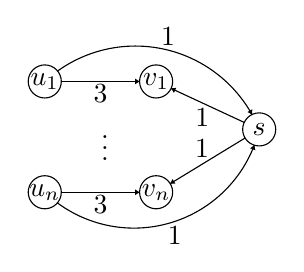
\begin{tikzpicture}[scale=0.07]
\tikzstyle{every node}+=[inner sep=0pt]
\draw [black] (18.5,-12.8) circle (3);
\draw (18.5,-12.8) node {$u_1$};
\draw [black] (38.7,-12.8) circle (3);
\draw (38.7,-12.8) node {$v_1$};
\draw [black] (18.5,-32.9) circle (3);
\draw (18.5,-32.9) node {$u_n$};
\draw [black] (38.7,-32.9) circle (3);
\draw (38.7,-32.9) node {$v_n$};
\draw (29.4,-23.4) node {$\vdots$} ;
\draw [black] (57.4,-21.5) circle (3);
\draw (57.4,-21.5) node {$s$};
\draw [black] (21.5,-12.8) -- (35.7,-12.8);
\fill [black] (35.7,-12.8) -- (34.9,-12.3) -- (34.9,-13.3);
\draw (28.6,-13.3) node [below] {$3$};
\draw [black] (21.5,-32.9) -- (35.7,-32.9);
\fill [black] (35.7,-32.9) -- (34.9,-32.4) -- (34.9,-33.4);
\draw (28.6,-33.4) node [below] {$3$};
\draw [black] (20.825,-10.907) arc (125.59934:29.18714:24.243);
\fill [black] (56.1,-18.8) -- (56.15,-17.85) -- (55.28,-18.34);
\draw (40.87,-6.38) node [above] {$1$};
\draw [black] (56.513,-24.364) arc (-20.88164:-126.45095:23.371);
\fill [black] (56.51,-24.36) -- (55.76,-24.93) -- (56.7,-25.29);
\draw (42.07,-39.01) node [below] {$1$};
\draw [black] (54.84,-23.06) -- (41.26,-31.34);
\fill [black] (41.26,-31.34) -- (42.2,-31.35) -- (41.68,-30.5);
\draw (47.05,-26.7) node [above] {$1$};
\draw [black] (54.68,-20.23) -- (41.42,-14.07);
\fill [black] (41.42,-14.07) -- (41.93,-14.86) -- (42.36,-13.95);
\draw (47.07,-17.66) node [below] {$1$};
\end{tikzpicture}
\end{center}
	\caption{Graph with small HD but large CHD: The graph comprises $2n+1$ nodes, with the edge labels representing the lengths. Note that the shortest paths in the graph are of the form $sv_i$, $u_is$ and $u_isv_j$ (for all combinations $i,j$). Thus, the HD is $1$ as $H_{v,r}=\crl{s}$ is a hitting set for all these paths. On the other hand, if we have costs such that $c(u_iv_i)=0\,\forall\,i$, while all other edges have cost $1$, then we have $n$ parallel efficient paths $u_iv_i$, which must all be hit by any EPHS.}
	\label{fig:big_chd}
\end{figure}
\begin{proposition}\label[proposition]{prop:example_bad_chd}
	There are networks with HD $1$ where the CHD, and also the sparsity of an EPHS, is $n$.
\end{proposition}
\begin{proof}
	Consider the directed graph $G$ defined in Figure~\ref{fig:big_chd}.
	It is easy to see that $H_{v,r}=\crl{s}$ is a shortest-path hitting set for every $r>0$ and $v\in V(G)$; hence the HD is $1$.
	On the other hand, suppose the costs are such that $c(u_iv_i)=0$ for every $i$, while all other costs are set to $1$.
	Note that the $1$-significant efficent paths intersecting the ball $B_s(2)$ are $u_iv_i$, which are all disjoint.
	Therefore, the hitting set $H_{s,1}$ must contain at least $n$ elements. Moreover, the same argument shows that the sparsity of the best LSHS for $\PS$ is $1$, whereas the sparsity of \emph{any} EPHS is also lower bounded by $n$.
\end{proof}

\begin{remark}
	One criticism of the graph in \cref{fig:big_chd} is that it has a maximum degree of $n$.
	However, the result holds even for bounded degree graphs.
	See \cite{TechReport} for a more involved example showing this.
	%In \cref{app:generalhd}, where we discuss alternative notions of HD, we give a more involved example with bounded degrees that exhibits the same separation between LSHS and EPHS for even stronger notions of HD.
\end{remark}

Intuitively, the separation between HD and CHD (or more particularly, the hub labels for computing SPs and CSPs) occurs due to the fact that, for arbitrary graphs and cost functions, the shortest and efficient paths may be completely unrelated. 
For real-world networks, however, this appears unlikely.
In particular, intuition suggests that efficient paths largely comprise of segments which are in fact shortest-paths in their own right. 
This notion can be formalized via the following definition of a \emph{partial witness} 
\begin{definition}[Partial Witness]
	Let $\beta\geq 0$.
	We say that a path system $\calQ$ is $\beta$-witnessed by the path system $\calQ'$ if, for every $Q\in\calQ$, $\exists Q'\in\calQ'$ such that $Q'\subseteq Q$ and $\ell(Q')\geq 2^{-\beta}\ell(Q)$.
\end{definition}
We can now ask if the hub labels for computing SPs and CSPs can be related in settings where the shortest-path system $\PS$ is a partial witness for the efficient path system $\PE$.
At an intuitive level, the partial witness property says that efficient and shortest paths are not completely different, i.e., if $Q$ is efficient, a fraction $2^{-\beta}$ of $Q$ is a SP.
As a consequence, a node hitting numerous paths in $\PS$, should also hit many paths in $\PE$.
Note that asking for the witness property to hold for all lengths is too extreme, as this essentially requires that all single-hop paths with 0 costs are shortest paths.
Thus, we want this property only for `long-enough' paths. 

We now show that if, for some $\beta$, the network indeed has the partial witness property for paths longer than some $r_\beta$, then we can relate the HL sizes for the two problems in terms of $\beta$ and the doubling dimension $\alpha$. 
Note that the doubling dimension depends on $G$ and $\ell$; the partial witness property depends on the interplay between $G$, $c$ and $\ell$.
Observe also that, if $\alpha$ is a constant, then the requirement in \cref{theo:witness_doubling} is for paths longer than $r_\beta\sim h\alpha^{\beta-2}$.
\begin{theorem}\label{theo:witness_doubling}
	Assume $G$ is $\alpha$-doubling and $\PE_r$ is $\beta$-witnessed by $\PS$ for every $r\geq r_\beta$, where $r_\beta=2^{\log_\alpha(\alpha^{\beta-2} h)}$. 
	Then, for any $r>0$, given an $(h,r)$-LSHS, we can construct, in polynomial time, an $(\alpha^{\beta} h,r)$-EPHS for $(G,\ell,c)$. 
\end{theorem}

\begin{proof}
	For any $r$, we need to construct a hitting set $C^E$ for $\PE_r$.
	Assume first $r\geq r_\beta$.
	Take $C$ as the hitting set for $\PS_{2^{-\beta}r}$, which is guaranteed to be sparse with respect to balls of radius $2^{-\beta+1}r$.
	Define the desired set by
	\[
	C^E\defeq\{v\in C: v \text{ is in some $r$-efficient path} \}.
	\]
	
	Since $\PS$ is a $2^{-\beta}$-witness for $\PE_r$, $C^E$ is indeed a hitting set for $\PE_r$.
	We are only left to prove the sparsity.
	Take some $u\in V$, by doubling dimension we can cover $\Bf_{2r}(u)$ by at most $\alpha^\beta$ balls of radius $2^{-\beta+1}r$.
	Each of these balls contains at most $h$ elements of $C$, therefore the sparsity is as claimed.
	The argument for reverse balls is identical.
	
	Now we analyse the case $r< r_\beta$.
	It is no longer true that efficient paths are witnessed, but now the neigborhoods are small.
	We first claim that, for any $v\in V$ and $r>0$, $\abs{B_{r}(v)}\leq \alpha^{\log_2r+1}$.
	Indeed, using the doubling property $\log_2r+1$ times, we can cover $B_r(v)$ with balls of radii $1/2$.
	Since the minimum edge length is $1$, all of these balls must be singletons and the claim follows.
	Now we can take $C=V$ as the EPHS.
	Clearly $C$ hits all the paths and the local sparsity is at most the size of the ball.
	Using our assumption on $r_\beta$, a simple computation shows that $\card{B_{2r}(v)}\leq \alpha^{\log_2r_\beta+2}\leq h\alpha^\beta$. 
\end{proof}
\begin{remark}
	The existence of a $\beta$-witness is not enough to bound the CHD. 
	Nevertheless, as we discuss in Section~\ref{ssec:hldef}, the existence of $(h,r)$-LSHS already allows the construction of HL. 
	%Moreover, the above argument does indeed give a bound for a weaker definition of HD (details in \cite{TechReport}).
\end{remark}
%\begin{remark}
%In order to make it more transparent, we state the above result in terms of $\alpha$ and $h$. 
%However, these quantities are somewhat related; it can be shown that $\alpha\leq 2h\Delta+1$ (cf.~\cite{skeleton}).
%\end{remark}
